\documentclass{article}
    % General document formatting
    \usepackage[margin=0.7in]{geometry}
    \usepackage[parfill]{parskip}
    \usepackage[utf8]{inputenc}
    \usepackage{graphicx}
    \usepackage[sort&compress,numbers,super]{natbib}
    \usepackage{booktabs}
    
    % Related to math
    \usepackage{amsmath,amssymb,amsfonts,amsthm}
\begin{document}
\chapter{Localized Intrinsic Valence Virtual Orbitals as a Tool for the Automatic Classification of Core Excited States}
\epigraph{\textit{``We must be clear that when it comes to atoms, language can be used only as in poetry. The poet, too, is not nearly so concerned with describing facts as with creating images and establishing mental connections''}}{Niels H. D. Bohr}
\begin{chapabstract}
Accurate assignments of the unoccupied molecular orbitals involved in electronic excited states are crucial to the interpretation of experimental spectra. Here we present an automated approach to the assignment of excited states by introducing a unique orbital basis known as localized intrinsic valence virtual orbitals (LIVVOs), which are a special case of the previously reported valence virtual orbitals. The LIVVOs are used to quantify the local contributions to particle orbitals from orthogonality-constrained density functional theory, providing an assignment with atomic-level/angular momentum shell specificity. This localized set also allows us to define the total valence character of an excited state. We highlight the utility of our approach by studying the local orbital changes in core-excited states at the sulfur K-edge of ethanethiol and benzenethiol as well as hydrogen bonding in the water dimer.
\end{chapabstract}
% Introduction
\section{Introduction}
Any interpretation of electronic spectroscopy depends upon assigning spectral features of the experimental spectrum to discrete electronic transitions calculated using excited state quantum chemistry methods. This requires characterization of the molecular orbitals involved in the discrete transition. Transitions are usually assigned by visual inspection of the contributing virtual molecular orbitals (MOs). Often, when these MOs do not have well defined character, orbital labels are used instead (e.g. LUMO, LUMO + 1, etc.). These approaches are somewhat unsatisfactory. The assignment of orbital character based on MO plots is potentially ambiguous. Furthermore, characterizing a transition using orbital labels is problematic because virtual orbitals are not uniquely defined and they strongly depend on the basis set and level of theory employed. 

A unique branch of electronic spectroscopy involving the excitation of core electrons using X-ray photons called near-edge X-ray absorption fine structure (NEXAFS) spectroscopy has garnered particular interest due to advancements in high-resolution tunable synchrotron light sources. NEXAFS spectroscopy has become an indispensable experimental tool for probing local electronic and geometrical information in a wide variety of molecular systems. \cite{westre_multiplet_1997,loble_covalency_2015-1,idrees_oxidation_2014,nelson_introduction_2012-1} The significant features of the NEXAFS spectrum arise from core orbital to unoccupied valence orbital transitions. \cite{stohr_nexafs_1992-1} The atomic nature of the core orbitals involved in these transitions (1s, 2s, 2p, etc.) makes NEXAFS a spectroscopic technique for elucidating local electronic structure information. Quantum chemistry calculations serve as a vital tool for gleaning meaningful electronic structure information from NEXAFS spectra including the nature of unoccupied orbitals, orbital mixing effects, and covalent character.\cite{stohr_nexafs_1992-1,loble_covalency_2015-1,nelson_introduction_2012,milne_recent_2014-1,cabaret_first-principles_2010-1}
A myriad of theoretical methods have been developed for the computation of core-excited states, ranging from rigorous methods focused on high accuracy \cite{coriani_coupled-cluster_2012,nooijen_description_1995,besley_equation_2012,peng_energy-specific_2015-1,dutta_intermediate_2014-1,brabec_communication:_2012,sen_study_2013-1,schirmer_beyond_1982-2,salpeter_relativistic_1951-1,barth_theoretical_1980,butscher_all-electron_1977-1,roemelt_excited_2013,asmuruf_calculation_2008,grimme_density_1996,lopata_linear-response_2012-2,fernando_x-ray_2015}
to computationally efficient methods focused on applications to larger systems.\cite{rehr_theoretical_2000,natoli_multiple_2012-1,joly_x-ray_2001,lowdin_statistical_1972,stener_time_2003-1,besley_time-dependent_2010-2,lestrange_calibration_2015,kuramoto_theoretical_2005,ohtsuka_inner-shell_2006,kolczewski_detailed_2001-1} The primary motivation underpinning these theoretical developments has been to obtain more accurate excitation energies and/or oscillator strengths. In contrast, the character of the wave function is analyzed in a more cursory fashion.

A recent work by the group of Dreuw\cite{wenzel_physical_2016,plasser_new_2014,plasser_new_2014-1} has taken a significant step toward a more rigorous description of core-excited states.
Using the one-particle transition density matrix and the one-particle difference density matrix, these authors were able to quantify the effects of relaxation, estimate multireference character, and provide information on the exciton size. These methods are a significant step toward a robust characterization of excited-states.
Myhre, Coriani, and Koch\cite{myhre_near-edge_2016} also recently used visualization of the one-particle difference density matrix in order to track the localization of core-excited states, relying on analysis of the excitation amplitudes of coupled cluster response calculations to assign the character of core-valence transitions. Although a fair amount of attention has been put forth to add a breadth of different descriptors for excited states, little attention has been put toward trying to improve upon the method of assigning orbital character.

Canonical molecular orbitals often complicate the assignment process because valence virtual MOs are mixed with polarization and diffuse functions included in the basis set.
A common approach to obtain more chemically meaningful valence orbitals is to project the virtual space onto a set of atomic valence orbitals. This approach hinges on the assumption that valence atomic orbitals are the dominant contributors to the valence molecular orbitals. This assumption was justified in the 1980s by Rudenberg and coworkers by obtaining overlaps close to unity between free-atom AOs and their projection onto the molecular orbitals of MCSCF wave functions. \cite{ruedenberg_are_1982}
Perhaps, the most popular method to analyze wave functions in terms of atomic valence contributions is Weinhold's natural atomic/bond orbital (NAO/NBO) analysis.\cite{foster_natural_1980,reed_natural_1985} This method partitions the full density matrix into atomic sub-blocks that are diagonalized in order to produce atom-localized hybrid valence orbitals.
AO projection based methods have been presented throughout the literature including polarized atomic orbitals, \cite{lee_extracting_2000-1,subotnik_fast_2005} enveloping localized orbitals,\cite{auer_dynamically_2006-1} intrinsic minimal atomic basis orbitals,\cite{laikov_intrinsic_2011-1} molecule-adapted atomic orbitals, \cite{szczepanik_minimal_2013-1} and intrinsic atomic orbitals. \cite{knizia_intrinsic_2013}
The approach presented in this work is based on the valence virtual orbitals (VVOs) scheme. \cite{lu_molecule_2004}
VVOs are built by bringing virtual valence MOs into maximum coincidence with a minimal atomic basis set via a unitary transformation.
The VVOs have been used with success to identify the valence LUMO in a variety of molecular systems,\cite{schmidt_valence_2015} to characterize bond breaking/formation along dissociation pathways,\cite{west_comprehensive_2015-1} and as a set of starting orbitals for multi-configurational SCF calculations.\cite{west_comprehensive_2013} VVOs can be easily localized and provide an accurate representation of the localized valence antibonding orbitals in a molecule. 

In this work we report a new method for automated classification of virtual orbitals in electronic excited states by quantifying the local contributions using a localized set of VVOs.
To generate the VVOs an accurate atomic minimal basis set (AAMBS) that spans the atomic valence space is required. We propose to represent the AAMBS using a minimal basis set of quasiatomic orbitals.\cite{lu_molecule_2004}
These are generated using projection operators according to Knizia's intrinsic atomic orbitals (IAOs) procedure\cite{knizia_intrinsic_2013} and localized using the Pipek--Mezey localization scheme. \cite{pipek_fast_1989}
The combination of VVOs projected onto a localized intrinsic orbital basis is abbreviated as LIVVOs.
To compute excitation energies we employ our recently proposed orthogonality-constrained DFT (OCDFT) approach\cite{evangelista_orthogonality_2013} to compute a manifold of states.\cite{derricotte_simulation_2015}
OCDFT is a variational time-independent DFT method built upon a generalized Kohn-Sham scheme.
In OCDFT excited state energies are approximated by a Kohn--Sham procedure augmented with orthogonality constraints between ground and excited state wave functions.

This new classification method is applied to the core-excited states involved in NEXAFS spectroscopy. We utilize the quantification of local contributions to analyze substituent effects in  thiols (ethanethiol, benzenethiol) and intermolecular interactions in the water dimer. The thiols were chosen as an example of molecules where the relevant excited states have significant contributions from more than one valence antibonding MO. Previous studies have not fully characterized the antibonding character of orbitals involved in core-valence excitations.\cite{behyan_chemical_2014,behyan_sulfur_2013,behyan_sulfur_2011}  We show that we are able to provide insight into the nature of these excited states using LIVVOs. Hydrogen bonding interactions in water have received plenty of attention within the X-ray absorption community.\cite{wernet_structure_2004,cavalleri_interpretation_2002,smith_probing_2006,prendergast_x-ray_2006-2,iannuzzi_x-ray_2008,leetmaa_theoretical_2010,kuhne_nature_2014}
Studies have shown that NEXAFS spectral changes upon the formation of a hydrogen bond is a result of localization of excited states along either the free OH bond or the hydrogen bond.\cite{smith_probing_2006,prendergast_x-ray_2006-2,kuhne_nature_2014,tse_x-ray_2008,smith_energetics_2004,smith_response_2005,chen_x-ray_2010,clark_structure_2010,vinson_theoretical_2012}
However, the degree of localization has not been quantified.  In this work we show that LIVVOs help quantify the localization of core excited states of the water dimer and that this metric is correlated some some spectral features.

%
% Theory 
%
\section{Theory}

\begin{figure*}[h!]
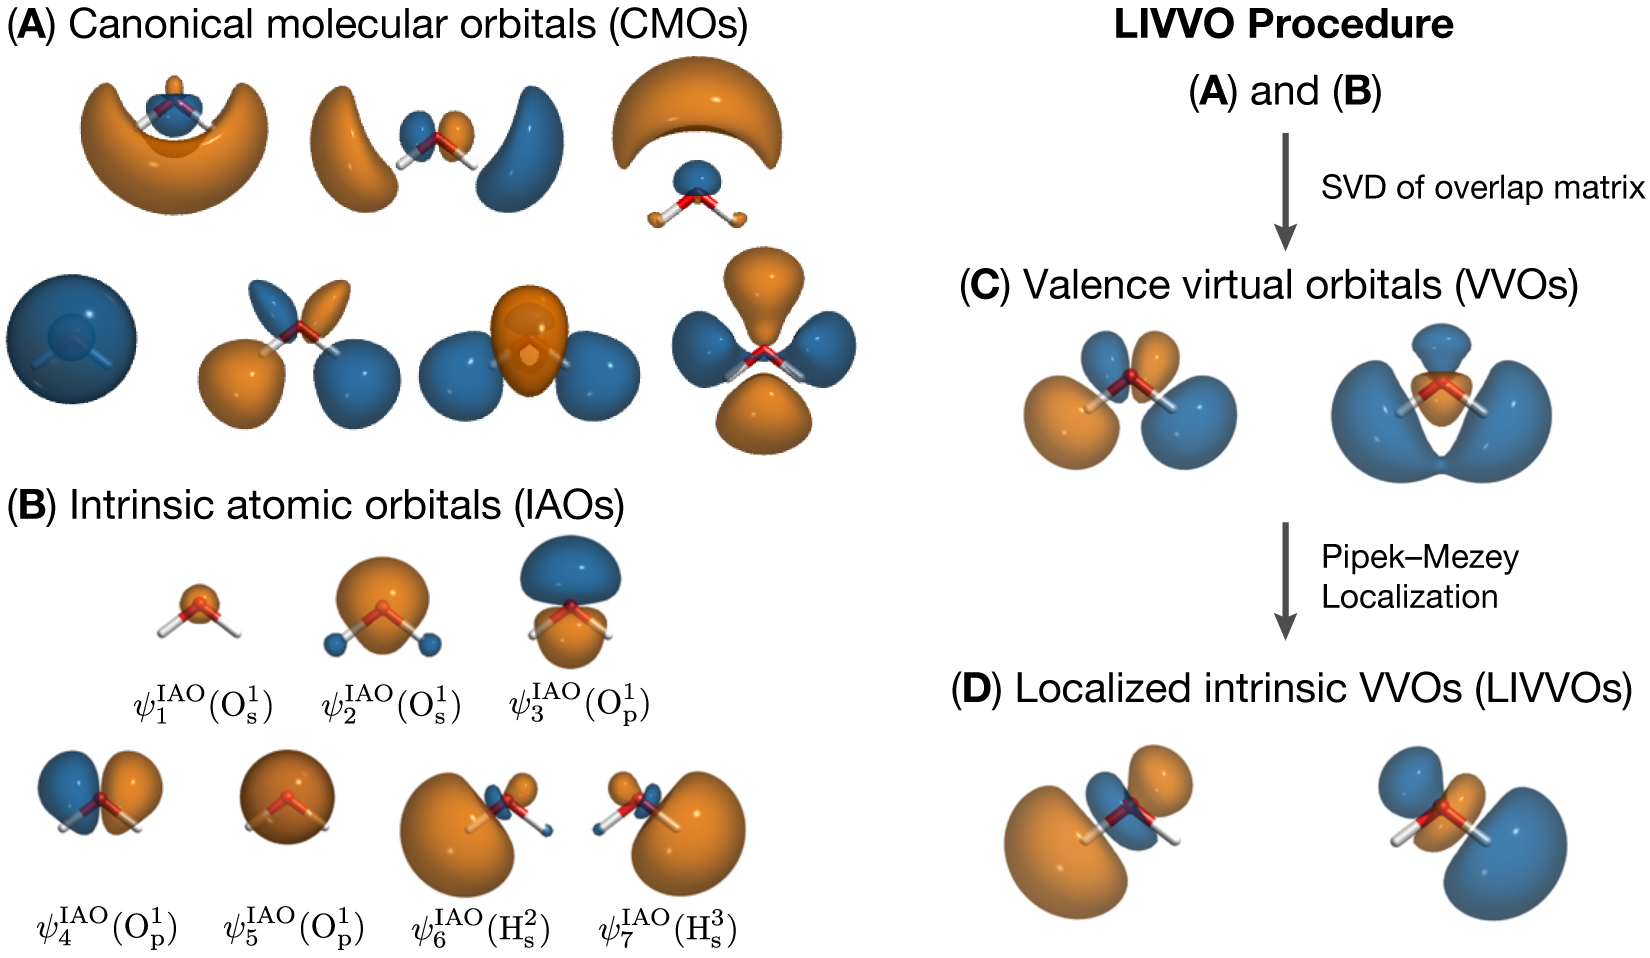
\includegraphics[width=5.5in]{figure_1_vvo_localization.png}
\caption{Illustration of the procedure used to construct localized intrinsic valence virtual orbitals (LIVVOs). (A) Canonical molecular orbitals (CMOs) of water computed at the B3LYP/aug-cc-pVTZ level of theory. (B) Intrinsic atomic orbitals obtained from the CMOs of water and corresponding assignment to a given atom and angular momentum shell.
(C) Delocalized valence virtual orbitals (VVOs) obtained by singular value decomposition of the overlap matrix [eq~\eqref{eq:overlap}]. 
(D) Localized intrinsic valence virtual orbitals (LIVVOs) for water after Pipek-Mezey localization of the VVOs.}
\label{fig:vvo_localization}
\end{figure*}

In this section we discuss three aspects of our approach to analyze core excitations.
First, we consider the construction of the localized intrinsic valence virtual orbitals (LIVVOs) from canonical molecular orbitals (CMOs) and intrinsic atomic orbitals (IAOs).
Next, we discuss how to automate the determination of the atomic character of the  IAOs and the LIVVOs.
Finally, we discuss the procedure used to analyze the particle orbital in OCDFT computations of core-excited states.

\subsection{Construction of Localized Intrinsic Valence Virtual Orbitals}
Here we summarize the construction of VVOs and discuss how to obtain the LIVVOs.
The procedure outlined here is illustrated in Figure~\ref{fig:vvo_localization} for the case of water.
The construction of VVOs begins by first identifying the virtual subset of the canonical molecular orbitals ($\{ \phi_a\}$) from a ground state SCF calculation.
The virtual CMOs are expanded in an atom-centered basis $\{\chi_{\mu}\}$ and are expressed in terms of MO coefficients $C_{\mu a}$
\begin{align}
|\phi_a\rangle = \sum_{\mu}^{N_\mathrm{AO}} |\chi_{\mu} \rangle C_{\mu a}, \quad a = 1,\ldots,N_\mathrm{vir}
\end{align}
where $N_\mathrm{AO}$ and $N_\mathrm{vir}$ are the number of atomic and virtual orbitals, respectively.
As shown in Figure~\ref{fig:vvo_localization}A, the virtual CMOs may have contributions from diffuse functions and their valence character is difficult to interpret.

To identify the valence character of the CMOs, we perform a VVO analysis\cite{Lu:2004cw,Lu:2004gq,schmidt_valence_2015} using the intrinsic atomic orbitals (IAOs) of Knizia\cite{knizia_intrinsic_2013} as the underlying accurate atomic minimal basis set.
IAOs are a set of orthonormal polarized atomic orbitals that can exactly express the occupied molecular orbitals of the ground state Kohn-Sham (KS) determinant $| \Phi \rangle$.
IAOs are expressed in terms of the atomic orbital basis as
\begin{align}
|\psi_{\rho}^\mathrm{IAO}\rangle = \sum_{\mu}^{N_\mathrm{AO}} |\chi_{\mu} \rangle \tilde{C}_{\mu \rho}, \quad \rho = 1, \ldots, N_\mathrm{IAO}
\end{align}
where $\tilde{C}_{\mu \rho}$ is the IAO coefficient matrix and $N_\mathrm{IAO}$ is the number of IAO orbitals.
As shown in Figure~\ref{fig:vvo_localization}B, in the case of water there are 7 IAOs that correspond to the oxygen atom 1s, 2s, and 2p shells and a single 1s orbital for each hydrogen atom.

Next, the overlap matrix ($\mathbf{S}$) of the canonical virtual orbitals with the IAO  functions $\psi_{\rho}^\mathrm{IAO}$ is evaluated:
\begin{align} \label{eq:overlap}
(\mathbf{S})_{a\rho} = \langle \phi_a | \psi_{\rho}^\mathrm{IAO} \rangle
\end{align}
and as suggested in Ref. \citenum{schmidt_valence_2015} a singular value decomposition (SVD) is performed on $\mathbf{S}$:
\begin{align}
\mathbf{S} = \mathbf{U} \boldsymbol{
\sigma} \mathbf{V}^{\dagger}
\end{align}
to yield orthogonal transformation matrices ${\bf U}$ and ${\bf V}$.
These matrices are rotations of the virtual space and the IAO space, respectively, that bring the two sets of orbitals into maximum coincidence.
The number of VVOs ($N_{\rm VVO}$) is given by the number of IAOs minus the number of occupied molecular ($N_{\rm occ}$) orbitals: $N_{\rm VVO} = N_{\rm IAO} - N_{\rm occ}$.
Assuming that the singular value decomposition orders the singular values ($\sigma_v$) in descending order, then the VVOs are obtained by transforming the canonical virtual orbitals with the first $N_{\rm VVO}$ columns of the matrix $\mathbf{U}$:
\begin{equation}
\label{eq:orbital_rotation}
| \psi^{\rm VVO}_v \rangle = \sum_a^{N_\mathrm{vir}} | \phi_a \rangle U_{av}, \quad v = 1, \ldots, N_{\rm VVO}.
\end{equation}

The VVOs for water shown in Figure~\ref{fig:vvo_localization}C, have valence character and correspond to the plus and minus combination of localized $\sigma^*_\text{O--H}$ orbitals.
Following Pipek--Mezey localization,\cite{pipek_fast_1989} we arrive at a set of localized VVOs that span the antibonding interactions of the molecular environment. We refer to this localized set as localized intrinsic valence virtual orbitals (LIVVOs). In the case of water, when the VVOs are localized we obtain the $\sigma^*_\text{O--H}$ orbitals drawn in Figure~\ref{fig:vvo_localization}D.

\subsection{Determination of the character of the IAOs and LIVVOs}
The goal of our analysis is to express excited states using the LIVVO basis. In addition, we are also interested in determining the dominant atomic character of each excited state.
To this end, we have automated the analysis of the atomic character of the LIVVOs.
Our approach starts with the assignment of the atomic character of each IAO via a Mulliken population analysis.\cite{mulliken_electronic_1955,mulliken_electronic_1955-1}
For each IAO, $\psi_{\rho}^\mathrm{IAO}$, we compute the population matrix:
\begin{equation}
P_{\mu\nu}(\rho) = \tilde{C}_{\mu \rho} S_{\mu\nu} \tilde{C}_{\nu \rho}, \quad \rho = 1, \ldots, N_\mathrm{IAO}
\end{equation}
Gross populations on atom $A$ and angular momentum shell $l$ [GP$_{A_l}(\rho)$] are obtained as partial sums of the population matrix:
\begin{equation}
\mathrm{GP}_{A_{l}}(\rho)  = \sum_{\mu \in A_{l}} \sum_{\nu}^{N_\mathrm{AO}} P_{\mu\nu}(\rho) 
\end{equation}
where the sum over $\mu$ is restricted to all functions centered on atom $A$ with angular momentum quantum number  ${l}$.

Values of $\mathrm{GP}_{A_{l}}(\rho)$ for the water example are reported in Table \ref{tab:iao_atomic}.
The assignment of IAOs using the gross population is straightforward since there is always a dominant contribution from a single atom/shell.
For example, in the case of IAO $\psi^{\rm IAO}_6$, the largest contribution to $\mathrm{GP}_{A_{l}}(\rho)$ is from the H$_\mathrm{s}^2$ shell (1.18), followed by smaller contributions from the O$_\mathrm{s}^1$, O$_\mathrm{s}^1$, and H$_\mathrm{s}^3$ shells (with absolute value less or equal to 0.08).
Therefore, we define the character of $\psi_{\rho}^\mathrm{IAO}$ as the pair atom/shell ($A$,${l}$) for which $\mathrm{GP}_{A_{l}}(\rho)$ is maximum:
\begin{equation}
 \mathrm{character}(\psi_{\rho}^\mathrm{IAO}) = \arg\max_{(A,{l})} \mathrm{GP}_{A_{l}}(\rho) \label{eq:ioa_character}
\end{equation}
In the case of water, when eq~\eqref{eq:ioa_character} is applied to the IAOs we obtain the assignment reported in Figure~\ref{fig:vvo_localization}B.

\begin{table}[b]
\renewcommand{\arraystretch}{1.2}
\footnotesize
\centering
\caption{Atom-centered gross orbital populations [GP$_{A_l}(\rho)$] for the seven IAOs of water. Calculations were performed at the B3LYP/jun-cc-pVTZ level of theory.}
\begin{tabular}{r@{\hskip6pt}r@{\hskip6pt}r@{\hskip6pt}r@{\hskip6pt}r@{\hskip6pt}r@{\hskip6pt}r@{\hskip6pt}r}
\toprule
$A_{l}$ & $\psi^{\rm IAO}_1$ & $\psi^{\rm IAO}_2$ & $\psi^{\rm IAO}_3$ & $\psi^{\rm IAO}_4$& $\psi^{\rm IAO}_5$& $\psi^{\rm IAO}_6$& $\psi^{\rm IAO}_7$ \\[3pt]
\midrule
O$_\mathrm{s}^1$ & 1.00 & 1.16 & 0.00 & 0.00 & 0.00 & $-$0.08 & $-$0.08 \\
O$_\mathrm{p}^1$ & 0.00 & 0.00 & 1.04 & 1.11 & 1.00 & $-$0.07 & $-$0.07 \\
H$^2_\mathrm{s}$ &0.00 & $-$0.08 & $-$0.02 & $-$0.05 & 0.00 & 1.18&  $-$0.03\\
H$^3_\mathrm{s}$ & 0.00 & $-$0.08 & $-$0.02 & $-$0.05 & 0.00 & $-$0.03 & 1.18\\
\bottomrule
\end{tabular}
\label{tab:iao_atomic}
\end{table}
\setlength{\tabcolsep}{0.1em}

Once the atomic character of each IAO is determined, we characterize the atomic contributions to each LIVVO.
For each LIVVO, $\psi_l^{\rm LIVVO}$, we evaluate the overlap with all the IAOs ($\psi^{\rm IAO}_{\rho}$):
\begin{equation}
\label{eq:livvo_iao_overlap}
S'_{l \rho} = | \langle \psi_l^{\rm LIVVO} | \psi^{\rm IAO}_{\rho} \rangle |^2
\end{equation}
The initial step in classifying the LIVVOs is to determine their overall orbital character ($\sigma$,$\pi$,\ldots).
A LIVVO is classified as $\sigma^*$ if the largest elements of $S'_{l \rho}$ include contributions from IAOs with $s$ and $p$ character.
Similarly, a LIVVO is assigned $\pi^*$ character if the largest elements of $S'_{l \rho}$ arise exclusively from $p$-type IAOs.
The atoms involved in the LIVVO are identified by the character of the  largest elements of $S'_{l \rho}$.
For this purpose, we only include those IAOs whose overlap with a given LIVVO is greater than a threshold, which in the following examples is set to 0.1.

To illustrate this analysis we consider the case of acrolein ($\rm C_3H_4O$).
The following LIVVOs are characterized respectively as $\sigma^*_\text{C$^2$--C$^3$}$ and $\pi^*_\text{C$^2$--C$^3$}$:
\begin{equation*}
\begin{split}
\vcenter{\hbox{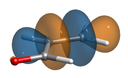
\includegraphics[width = 2.5cm]{img_1a}}} =& 
\, 0.20 \, \psi^{\rm IAO}(\rm C^2_s) + 0.24 \, \psi^{\rm IAO}(\rm C^2_p) \\
& + 0.20 \, \psi^{\rm IAO}(\rm C^3_s)  + 0.25 \, \psi^{\rm IAO}(\rm C^3_p) \\
\\
\vcenter{\hbox{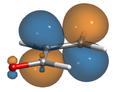
\includegraphics[width = 2.25cm]{img_1b}}} =& \,
 0.47 \, \psi^{\rm IAO}(\rm C^2_p)  + 0.51 \,  \psi^{\rm IAO}(\rm C^3_p)  
\end{split}
\end{equation*}
Note that the in the case of the $\sigma^*_\text{C$^2$--C$^3$}$ LIVVO there are contributions from both s and p orbitals, while 98\% of the $\pi^*_\text{C$^2$--C$^3$}$ LIVVO is comprised of p orbitals.
The construction and analysis of the LIVVOs is fully automated and is performed only once after a ground state KS computation.

\subsection{Analysis of OCDFT Particle Orbitals Using LIVVOs}
The procedure used to generate the LIVVOs relies only the information contained in the reference ground state determinant and is therefore applicable to any method.
The focus of this work is to apply the LIVVO to OCDFT computations of K-edge spectra.
First, we briefly summarize the features of OCDFT.
In OCDFT,\cite{evangelista_orthogonality_2013} a generalized Kohn--Sham picture is assumed, where to the $n$-th electronic state corresponds an auxiliary system of noninteracting electrons with wave function $\Phi^{(n)}$ and density $\rho^{(n)}$. The wave function for the auxiliary system is a single Slater determinant, $\ket{\Phi^{(n)}} = \ket[1]{\phi_1^{(n)}\phi_2^{(n)} \cdots\phi_N^{(n)}}$, where the set of orbitals $\{\phi_i^{(n)}\}$ are different for each electronic state. To avoid variational collapse, OCDFT enforces orthogonality conditions between all determinants:
\begin{equation}
\label{eq:OCcondition}
\langle \Phi^{(m)} | \Phi^{(n)} \rangle = \delta_{mn} \;\;\;  \forall m,n
\end{equation}

In this work we employ our constrained multiple hole/particle (CMHP) algorithm\cite{ayers_time-independent_2012} for the solution of multiple orthogonally constrained excited states.
The CMHP scheme fully accounts for relaxation of all orbitals, but rather than solving for the exact minimum orthogonality conditions, it imposes  sufficient orbital orthogonality conditions. Namely, we assume that the hole orbitals in core-excited states are localized and are orthogonal.
It follows then that one-electron excited states can be characterized by fully relaxed hole [$\phi_{\rm h}^{(n)}$] and particle [$\phi_{\rm p}^{(n)}$] orbitals, which span the occupied and virtual spaces of the ground state wave function, respectively.

For every excited state, we analyze the character of the particle orbital $\phi_{\rm p}^{(n)}$ by evaluating its overlap with each LIVVO ($\psi^{\rm LIVVO}_l$):
\begin{equation}
\label{eq:part_livvo_overlap}
\Omega_{\mathrm{p}l}^{(n)} = | \langle \phi^{(n)}_\mathrm{p} | \psi^{\rm LIVVO}_l \rangle |^2.
\end{equation}
The individual overlaps $\Omega_{\mathrm{p}l}^{(n)}$ are used to assign the character of the particle orbital to the $l$-th LIVVO.
In addition, we also define the total valence character $t^{\mathrm{val},(n)}_\mathrm{p} $ for any given particle orbital as the sum its overlap with all LIVVOs:
\begin{equation}
t^{\mathrm{val},(n)}_\mathrm{p} = \sum_{l}^{N_\mathrm{LIVVO}} \Omega_{\mathrm{p}l}^{(n)}.
\label{eq:total_valence_character}
\end{equation}
Since the LIVVOs give an accurate representation of valence orbitals in the molecule, it is possible to quantify the most important local contributions to the particle orbital. While this offers a very robust description for localized valence particle orbitals, it is important to note that the particle orbital describing the excited state can also be fairly diffuse with respect to the molecular environment. Such an orbital will obviously have relatively low overlap with the LIVVOs described here. This can be a desirable feature of our method as it allows for immediate identification of spectral contributions that arise from more diffuse orbitals. 
However, any further classification of the diffuse nature or Rydberg character of virtual orbitals is outside the scope of the current study.

\section{Computational Details}
OCDFT is currently implemented as a plugin for the PSI4 \cite{turney_psi4:_2012-1} \textit{ab initio} quantum chemistry package. All core excitation energies and oscillator strengths are obtained using the B3LYP \cite{lee_development_1988-1,becke_new_1993-3,vosko_accurate_1980-2,stephens_ab_1994-2} functional and a triple zeta correlation-consistent basis set jun-cc-pVTZ,\cite{woon_gaussian_1993-1,dunning_gaussian_1989-1} which is obtained by deleting diffuse functions from the highest subshell of every atom in the aug-cc-pVTZ basis set.\cite{papajak_perspectives_2011} The two-electron integrals are factorized using the density-fitting approximation\cite{dunlap_firstrow_1979,schrader_use_1962,baerends_self-consistent_1973,dunlap_robust_2000-1,dunlap_applicability_1977-1} with the jun-cc-pVTZ-JKFIT auxillary fitting basis.\cite{weigend_accurate_2006-2,weigend_hartreefock_2008}
Basis set dependence of the LIVVO analysis is investigated using the cc-pVXZ and aug-cc-pVXZ (X=D,T,Q) family of basis sets.\cite{kendall_electron_1992,dunning_gaussian_1989-1}
Intrinsic atomic orbitals were obtained using Robert Parrish's implementation in PSI4.\cite{Parrish:2014de}
The geometries for ethanethiol, benzenethiol, water monomer, and water dimer were all optimized at the B3LYP/aug-cc-pVTZ level of theory.

Peak intensities for each transition from the ground state to excited state ($n$) are based on the oscillator strength ($f_{\rm osc}$):
\begin{align}
f_{\rm osc} = \frac{2}{3}|\boldsymbol{\mu}_{n0}|^2\omega_n
\end{align}
where $\omega_n$ is the excitation energy calculated in OCDFT and $\boldsymbol{\mu}_{n0}$ is the transition dipole moment vector. OCDFT does not provide a direct route toward computation of the transition dipole moments, however, these can be approximated using the noninteracting Kohn--Sham determinants:
\begin{equation}
\boldsymbol{\mu}_{n0} = \langle \Phi^{(n)}|\mathbf{r}| \Phi^{(0)} \rangle
\label{eq:dipole}
\end{equation}
where $\Phi^{(n)}$ is the KS determinant for the $n$-th excited state and $\mathbf{r}$ is the position vector.
Spectroscopic broadening effects are simulated by representing each transition using a Gaussian lineshape with a FWHM of 0.4 eV.

\section{Results}
\subsection{Analysis of substituent effects in the spectra of thiols}

\begin{table*}[!t]
\renewcommand{\arraystretch}{1.2}
\centering
\footnotesize
\caption{Transition energies, oscillator strengths ($f_{\rm osc}$), and LIVVO assignments for all states calculated in the NEXAFS spectrum of ethanethiol and benzenethiol. Experimental energies and assignments are taken from Ref. \citenum{behyan_sulfur_2011}.}
\begin{tabular}{@{\extracolsep{6pt}}cccrcr@{}}
\toprule
& \multicolumn{3}{c}{OCDFT} & \multicolumn{2}{c}{Experiment} \\
\cline{2-4} \cline{5-6}
State & Energy (eV) & $f_{\rm osc}$ & LIVVO Assignment & Energy (eV)  & Assignment\\
\midrule
\multicolumn{6}{c}{\bf{Ethanethiol}} \\
1 & 2472.9 & 0.0022 & 58\% $\sigma^*_{\rm S^3-H^9}$ & 2472.2 & $\sigma^*_{\rm S-H}$ \\
& & & 22\% $\sigma^*_{\rm S^3-C^2}$\vspace{0.1cm} & & Weak $\sigma^*_{\rm S-C}$\\
2 & 2473.9 & 0.0011 & 57\% $\sigma^*_{\rm S^3-C^2}$ & 2473.1 & $\sigma^*_{\rm S-C}$ \\
& & & 18\% $\sigma^*_{\rm S^3-H^9}$\vspace{0.1cm} & &\\
3 & 2475.6 & 0.0004 & 9\% $\sigma^*_{\rm C^2-H^8}$ & 2474.9 & Poorly Defined \\
& & & 7\% $\sigma^*_{\rm C^2-H^7}$\vspace{0.1cm} & &\\
4 & 2476.2 & 0.0007 & 8\% $\sigma^*_{\rm S^3-C^2}$ & & \\
& & & 5\% $\sigma^*_{\rm C^2-H^8}$\vspace{0.1cm} & &\\
5 & 2476.1 & 0.0005 & 6\% $\sigma^*_{\rm C^1-H^6}$ & & \\
& & & 3\% $\sigma^*_{\rm C^2-H^7}$\vspace{0.1cm} & &\\
\multicolumn{6}{c}{\bf{Benzenethiol}} \\
1 & 2472.9 & 0.0023 & 61\% $\sigma^*_{\rm S^7-H^8}$ & 2472.4 & $\sigma^*_{\rm S-H}$\\
& & &  22\% $\sigma^*_{\rm S^7-C^3}$ & & Weak $\sigma^*_{\rm S-C}$ \vspace{0.1cm}\\
2 & 2474.2 & 0.0011 & 53\% $\sigma^*_{\rm S^7-C^3}$ & 2473.5  & Weak $\pi^*_{C=C}$ \\
& & & 16\% $\sigma^*_{\rm S^7-H^8}$\vspace{0.1cm} & &\\
3 & 2474.9 & 0.0001 & 68\% $\pi^*_{\rm C^{2,3,4}}$ & 2475.3 & $\sigma^*_{S-C}$ \\
& & & 15\% $\pi^*_{\rm C^{4,5,6}}$\vspace{0.1cm} & &\\
4 & 2475.3 & 0.0000 & 48\% $\pi^*_{\rm C^{1,2,6}}$ & &\\
& & & 34\% $\pi^*_{\rm C^{4,5,6}}$ & & \vspace{0.1cm}\\
5 & 2476.0& 0.0006 & 7\% $\sigma^*_{\rm S^7-H^8}$ & &\vspace{0.1cm}\\
\bottomrule
\end{tabular}
\label{tab:thiols}
\end{table*}





\begin{figure}[!b]
\centering
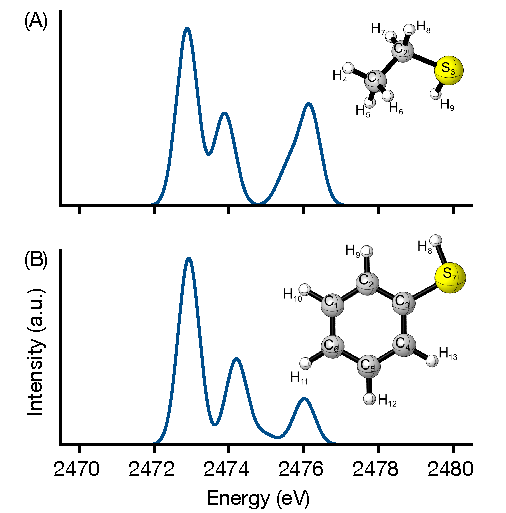
\includegraphics{figure_2_thiols_spectra.pdf}
\caption{Sulfur 1s near-edge x-ray absorption spectra of thiols calculated with OCDFT at the B3LYP/jun-cc-pVTZ level of theory. Spectra of (A) ethanethiol and (B) benzenethiol. Shown in the inset of each spectrum is the optimized structure for each molecule. Structures were plotted using CYLview software.\cite{legault_cylview_2009}}
\label{fig:thiols}
\end{figure}

\begin{figure*}[h]
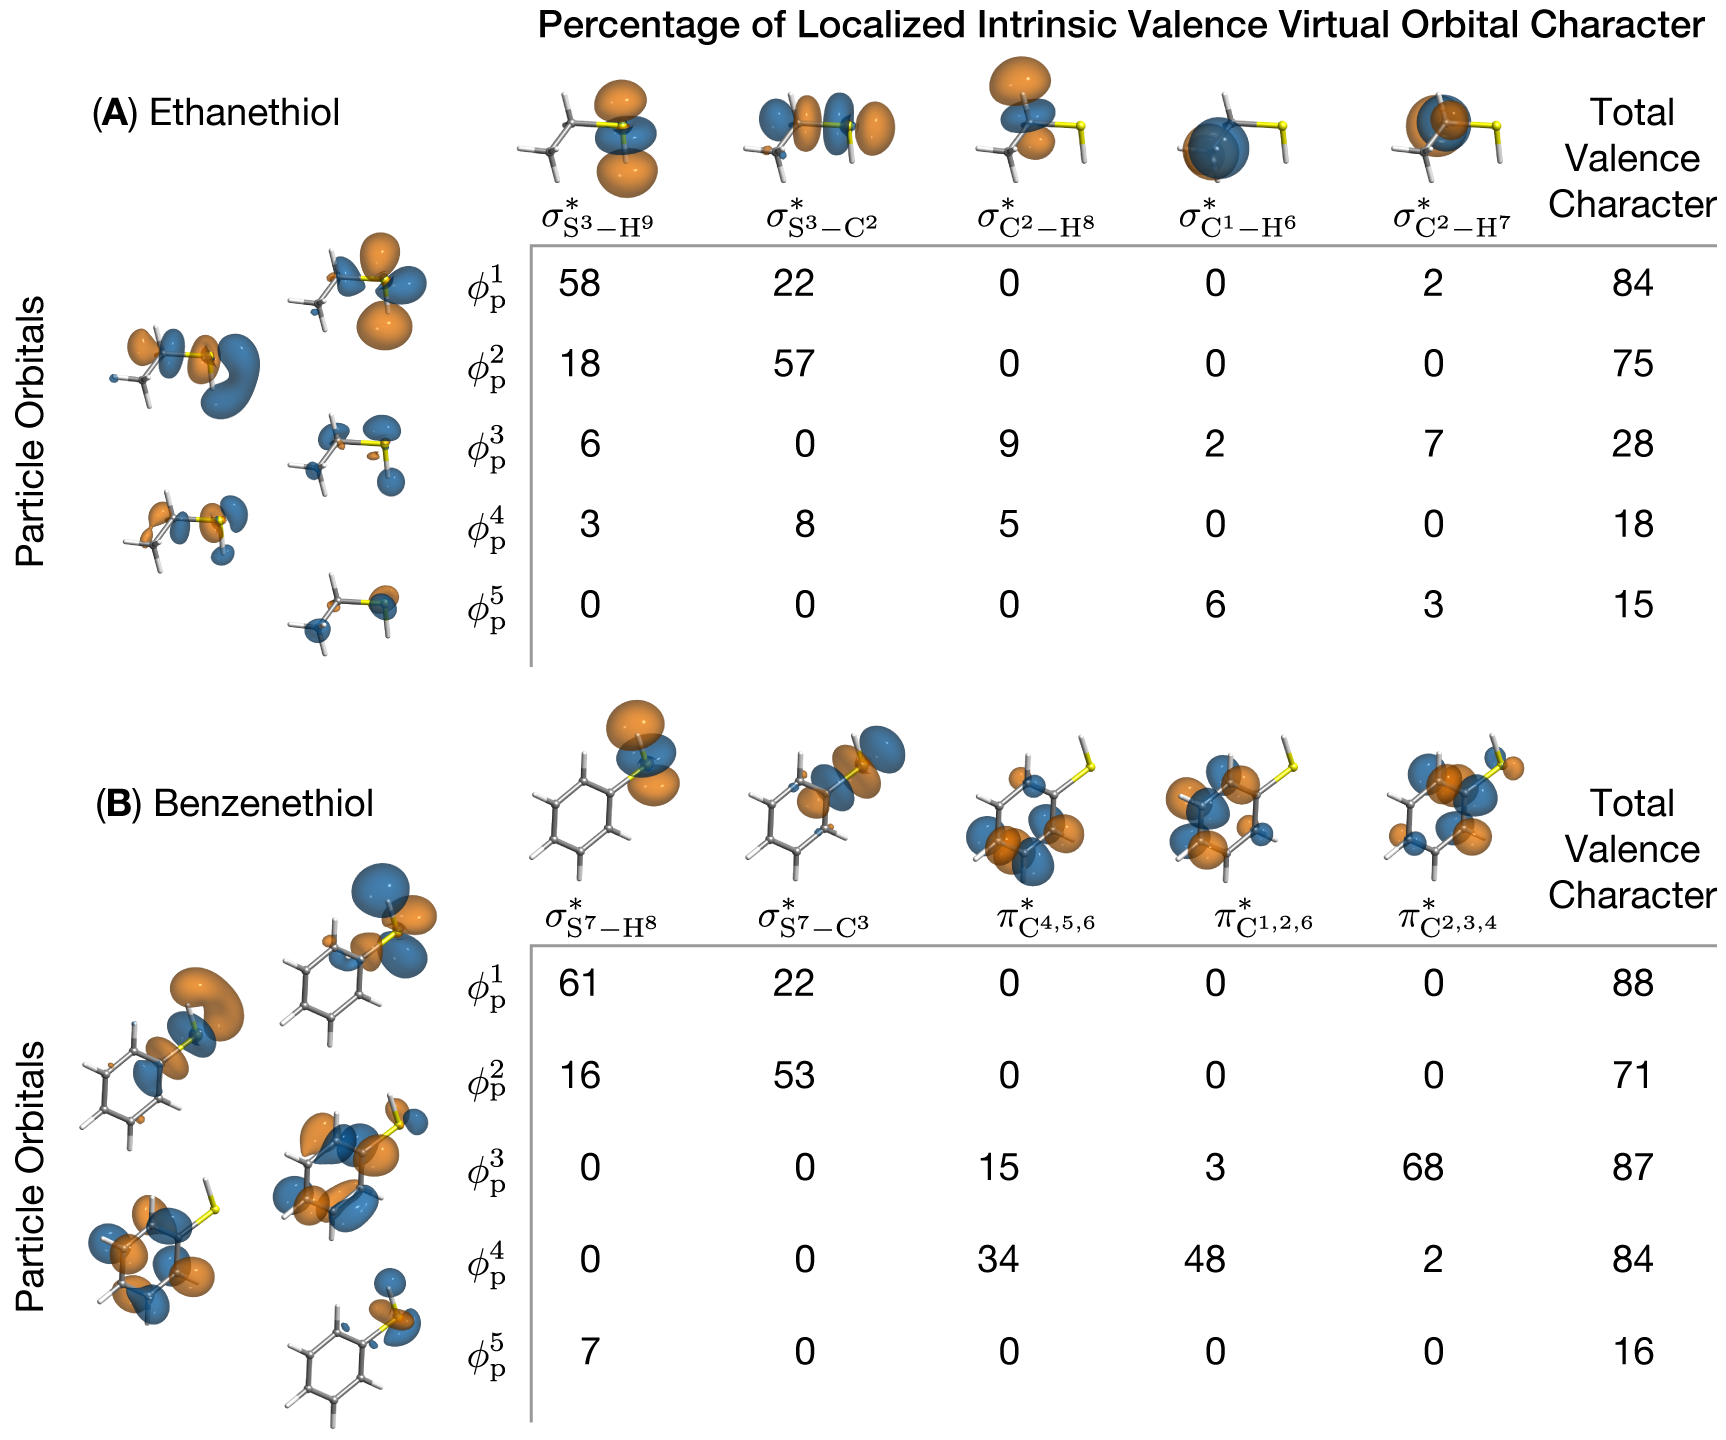
\includegraphics[width=5.75in]{figure_3_livvo_analysis_thiols.png}
\caption{Particle orbitals, valence virtual orbitals, and total valence character for each of the five core transitions in the NEXAFS spectrum of (A) ethanethiol (C$_2$H$_5$SH) and (B) benzenethiol (C$_6$H$_5$SH). Percentages shown represent the overlap of each particle orbital with the LIVVOs. Particle orbitals are numbered according to the calculated transitions reported in Table \ref{tab:thiols} while atom numberings correspond to those shown in Figure~\ref{fig:thiols}.}
\label{fig:thiols_cont}
\end{figure*}

Our first application of the LIVVO analysis for the classification of NEXAFS spectral features focuses on the effect of substituents on peak position and intensity.
In this section we compare the sulfur K-edge of ethanethiol (C$_2$H$_5$SH) and benzenethiol (C$_6$H$_5$SH).
The OCDFT NEXAFS spectra for these two compounds are shown in Figure~\ref{fig:thiols}.
Table \ref{tab:thiols} reports a comparison of experimental and theoretical excitation energies, OCDFT oscillator strengths, the LIVVO assignments, and total valence character for each state. 

The gas-phase experimental excitation energies shown in Table \ref{tab:thiols} for ethanethiol represents the three peaks of the spectrum at 2472.17, 2473.11, and 2474.87 eV. Our calculated OCDFT spectrum is also characterized by three peaks with transition energies that are in good agreement with the experimental spectrum. The first two are a result of strong single transitions at  2472.9 and 2473.9 eV. The final peak is a combination of three weak transitions that occur at 2475.6, 2476.2, and 2476.1 eV. 

The gas phase experimental spectrum of benzenethiol is characterized by three peaks at 2472.4, 2473.5, and 2475.3 eV. The theoretical spectrum has strong single transitions at 2472.9 eV and 2474.2 eV. The last peak is composed of weaker transitions at 2474.9, 2475.3, and 2476.0 eV.
In total, this gives us errors that are on average less than 1.0 eV across these two molecules. This agreement with the experimental spectrum is consistent with that seen in previous studies with OCDFT\cite{derricotte_simulation_2015,verma_predicting_2016} and are obtained without application of shifts to match experimental values.

By analyzing the overlap of the particle orbitals with all orbitals in the LIVVO basis, it is possible to quantify the degree of localization along each bond and discern the origin of some features of the ethanethiol and benzenethiol spectra.
The lowest energy transition in the NEXAFS spectrum of ethanethiol and benzenethiol occurs at  at 2472.9 eV, and was attributed mostly to a S 1s $\rightarrow$ $\sigma^*_\text{S--H}$ transition with a ``weak'' contribution from a S 1$s$ $\rightarrow$ $\sigma^*_\text{S--C}$ transition.\cite{behyan_sulfur_2013}
The LIVVO assignments, displayed in Figure~\ref{fig:thiols_cont}, show that in both cases the first state (corresponding to the particle orbital $\phi_\mathrm{p}^1$) can be assigned to $\sigma^*_\text{S--H}$ (50\%) and $\sigma^*_\text{S--C}$ (22\%) character. Going from ethanethiol to benzenethiol there is a slight increase in the degree of localization along the thiol bond. This is evidenced by the $\sigma^*_\text{S--H}$ character of the first excited state increasing from 58\% in ethanethiol, to 61\% in benzenethiol.

The second peak in the NEXAFS spectra of the thiols occurs at 2473.9 eV for  ethanethiol and at 2474.2 eV for benzenethiol. Again in this case, simple inspection of the particle orbitals ($\phi_\mathrm{p}^2$) shows orbital character along both the S--H and S--C bonds. The LIVVO assignments show that over 50\% of the character of the particle orbital can be assigned to the $\sigma^*_{\rm S-C}$ orbital in each molecule, while less than 19\% can be assigned to the $\sigma^*_{\rm S-H}$ orbital. Comparing our results with a previous study\cite{behyan_sulfur_2013} that employed the Hartree--Fock static exchange (HF-STEX) method, \cite{otero_nitrogen_2006,cooney_chemical_2004,urquhart_core_1997,urquhart_probing_1998,urquhart_near-edge_1999,kosugi_rydberg_1995} our assignments agrees well for the case of ethanethiol.
However, the OCDFT assignment is at odds with their assignment for benzenethiol where they attributed this peak feature to core transitions to $\pi^*$ orbitals associated with the phenol ring. The discrepency in this assignment likely stems from the differences in the energy ordering of the virtual orbitals between HF and DFT.

The third peak in the spectrum for both thiols is a combination of three low-intensity transitions. Of these, the most intense transition is predicted by OCDFT to be at 2476.2 eV for ethanethiol and 2476.0 eV for benzenethiol and corresponds to the particle orbital $\phi_\mathrm{p}^4$.
Considering the total valence characters shown in Figure~\ref{fig:thiols_cont} and the oscillator strengths shown in Table \ref{tab:thiols}, we see a clear trend relating the valence character and the oscillator strength of the transition.
In the case of ethanethiol, the low valence character of the transitions (28\% or lower) suggests that the smaller oscillator strength of the third peak is due to the diffuse mixed Rydberg character of particle orbitals $\phi_\mathrm{p}^3$, $\phi_\mathrm{p}^4$, and $\phi_\mathrm{p}^5$.

In the case of benzenethiol, the valence character of states $\phi_\mathrm{p}^3$ and $\phi_\mathrm{p}^4$ is high (87\% and 84\%, respectively) but these orbitals are mostly localized on the phenyl ring and give small contributions to the transition dipole moment.
State $\phi_\mathrm{p}^3$ is a mixture of $\pi^*_{\mathrm{C}^{2,3,4}}$ and $\pi^*_{\mathrm{C}^{4,5,6}}$ at 68\% and 15\% respectively, while state $\phi_\mathrm{p}^4$ is a mixture of $\pi^*_{\mathrm{C}^{1,2,6}}$ and $\pi^*_{\mathrm{C}^{4,5,6}}$ at 48\% and 34\% respectively.
This analysis suggests that the small overlap of these states with the sulfur atom is the cause of the small intensity of the corresponding transitions.
State $\phi_\mathrm{p}^5$ of benzenethiol has a much lower total valence character (16\%), however, since it has 7\% overlap with the $\sigma^*_{\rm S-H}$ thiol bond orbital, the corresponding transition still has a modest intensity.
We should note that thanks to the LIVVO analysis we were able to quantify the weak local contributions to the states that contribute to the third peak.
Previous studies\cite{behyan_sulfur_2013} were unable to assess the orbital character of this set of transitions.

\subsection{Signatures of hydrogen bonding in the NEXAFS spectrum of the water dimer}

\begin{table}[!t]
\renewcommand{\arraystretch}{1.2}
\centering
\footnotesize
\caption{Transition energies, oscillator strengths ($f_{\rm osc}$), and LIVVO assignments for all states calculated in the NEXAFS spectrum of the water monomer, dimer-A, and dimer-D.}
\begin{tabular}{@{\extracolsep{6pt}}cccr@{}}
\toprule
State & Energy (eV) & $f_{\rm osc}$ & LIVVO Assignment\\
\midrule
\multicolumn{4}{c}{\bf{Monomer}} \\
1 & 533.7 & 0.00811 & 42\% $\sigma^*_{\rm O_1-H_2}$ \\
 & & & 42\% $\sigma^*_{\rm O_1-H_3}$ \\
 2 & 535.4 & 0.01839 & 38\% $\sigma^*_{\rm O_1-H_2}$ \\
 & & & 38\% $\sigma^*_{\rm O_1-H_3}$ \\
 3 & 537.3 & 0.00786 & Rydberg/Diffuse \\
 4 & 537.8 & 0.00252 & Rydberg/Diffuse \\
 5 & 538.5 & 0.00167 & 6\% $\sigma^*_{\rm O_1-H_2}$ \\
 & & & 6\% $\sigma^*_{\rm O_1-H_3}$ \\
 \multicolumn{4}{c}{\bf{Dimer-A}} \\
 1 & 534.0 & 0.00737 & 41\% $\sigma^*_{\rm O_1-H_2}$ \\
 & & & 41\% $\sigma^*_{\rm O_1-H_3}$ \\
  2 & 535.8 & 0.01862 & 39\% $\sigma^*_{\rm O_1-H_2}$ \\
 & & & 39\% $\sigma^*_{\rm O_1-H_3}$ \\
   3 & 537.7 & 0.00552 & 14\% $\sigma^*_{\rm O_4-H_5}$ \\
 & & & 9\% $\sigma^*_{\rm O_4-H_6}$ \\
   4 & 537.9 & 0.00529 & 4\% $\sigma^*_{\rm O_4-H_6}$ \\
 & & & 3\% $\sigma^*_{\rm O_4-H_5}$ \\
   5 & 539.3 & 0.00282 & 12\% $\sigma^*_{\rm O_4-H_6}$ \\
 & & & 8\% $\sigma^*_{\rm O_4-H_5}$ \\
  \multicolumn{4}{c}{\bf{Dimer-D}} \\
 1 & 533.5 & 0.00605 & 52\% $\sigma^*_{\rm O_4-H_6}$ \\
 & & & 16\% $\sigma^*_{\rm O_4-H_5}$ \\
  2 & 534.9 & 0.00878 & 24\% $\sigma^*_{\rm O_4-H_6}$ \\
 & & & 18\% $\sigma^*_{\rm O_1-H_2}$ \\
   3 & 536.1 & 0.00574 & 3\% $\sigma^*_{\rm O_1-H_2}$ \\
 & & & 3\% $\sigma^*_{\rm O_1-H_3}$ \\
   4 & 536.6 & 0.00284 & 2\% $\sigma^*_{\rm O_4-H_5}$ \\
 & & & 2\% $\sigma^*_{\rm O_1-H_3}$ \\
   5 & 537.3 & 0.00623 & 25\% $\sigma^*_{\rm O_4-H_5}$ \\
 & & & 5\% $\sigma^*_{\rm O_4-H_5}$ \\
\bottomrule
\end{tabular}
\label{tab:water_spec}
\end{table}

Due to the critical role it plays in many processes in nature, hydrogen bonding is one of the most important noncovalent interactions in chemistry.\cite{morokuma_why_1977,kool_hydrogen_2001,fonseca_guerra_hydrogen_2000,stiopkin_hydrogen_2011,pflugrath_sulphate_1985}
The water dimer (H$_2$O)$_2$ is one of the simplest yet most important examples of hydrogen bonding in chemistry and has garnered plenty of attention from both theory and experiment. \cite{feyereisen_hydrogen_1996,kim_comparison_1994,reed_natural_1983,stevens_frozen_1987,szalewicz_theoretical_1988,headrick_spectral_2005,wang_multimode_2008,chng_experimental_2012,shank_accurate_2009,mukhopadhyay_water_2015,gomez_partition-dft_2017,zhang_quantitative_2017} This simple dimer is the basic building block of the structures of liquid water and ice, which have both been studied extensively with NEXAFS spectroscopy to uncover their underlying hydrogen bond coordination.\cite{wilson_x-ray_2001,wilson_characterization_2002,parent_structure_2002} A host of computational methods have been applied to study the effects of hydrogen bonding on the NEXAFS spectrum of water, including transition potential DFT (TPDFT), \cite{prendergast_x-ray_2006-2,iannuzzi_x-ray_2008,leetmaa_theoretical_2010,hetenyi_calculation_2004,cavalleri_half_2005} coupled-cluster singles and doubles (CCSD), \cite{coriani_coupled-cluster_2012,coriani_asymmetric-lanczos-chain-driven_2012,fransson_requirements_2016} and complex polarization propagator DFT (CPP-DFT). \cite{ekstrom_x-ray_2006} Here, we utilize our LIVVO analysis in order to quantify these effects on the NEXAFS spectrum.  


\textit{Water monomer}. 
A host of computational methods have been applied to study the effects of hydrogen bonding on the NEXAFS spectrum of water, including transition potential DFT (TPDFT), \cite{prendergast_x-ray_2006-2,iannuzzi_x-ray_2008,leetmaa_theoretical_2010,hetenyi_calculation_2004,cavalleri_half_2005} coupled-cluster singles and doubles (CCSD), \cite{coriani_coupled-cluster_2012,coriani_asymmetric-lanczos-chain-driven_2012,fransson_requirements_2016} and complex polarization propagator DFT (CPP-DFT). \cite{ekstrom_x-ray_2006}. Here, we utilize our LIVVO analysis in order to quantify these effects on the NEXAFS spectrum.  
Figure~\ref{fig:water_spec}A shows the NEXAFS spectrum for water monomer and the lowest-energy configuration of the water dimer.
To facilitate our analysis, we separate the dimer spectrum into contributions from the hole localized on the oxygen accepting the hydrogen bond (O$_1$, denoted as dimer-A) and a spectrum for the hole localized on the oxygen donating the hydrogen bond (O$_4$, denoted as dimer-D).
These partial contributions are shown in panels B and C of Figure~\ref{fig:water_spec}, respectively.
Table \ref{tab:water_spec} shows all of the calculated excitation energies, oscillator strengths and final LIVVO assignments for each state.

\begin{figure}[t!]
\centering
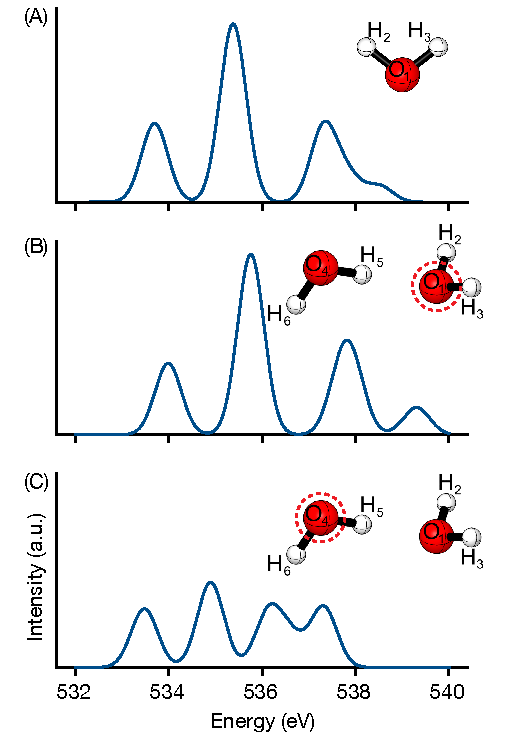
\includegraphics{figure_4_water_spectra.pdf}
\caption{Oxygen 1s Near-edge x-ray absorption spectra of: (A) water monomer, (B) dimer-A, and (C) dimer-D calculated with OCDFT at the B3LYP/jun-cc-pVTZ level of theory. Shown in the inset of each spectrum is the optimized structure for each molecule. For the water dimer, we indicate the core-excited atom with a red cicle. Structures were plotted using the CYLview software.\cite{legault_cylview_2009}}
\label{fig:water_spec}
\end{figure} 

The OCDFT computed NEXAFS spectrum of water monomer at the O K-edge, shown in Figure~\ref{fig:water_spec}, is defined by three characteristic peaks at 533.7, 535.4, and 537.3 eV respectively.
The positions of these peaks are in excellent agreement with the gas-phase experimental peak features which occur at 534.0, 535.9, and 537.0 eV. \cite{schirmer_k-shell_1993}
The first peak at 533.7 eV has a relative intensity of 0.44 and is characterized by the particle orbital $\phi^1_{\rm p}$ shown in Figure~\ref{fig:water_all_livvo}A, while the second peak at 535.4 is the most intense of the spectrum and is characterized by the particle orbital $\phi^2_{\rm p}$.
Two Rydberg transitions at 537.3 and 537.8 eV contribute to the third peak in the spectrum and are accompanied by a higher energy shoulder feature at 538.5 eV.

The water monomer particle orbitals are shown in Figure~\ref{fig:water_all_livvo}A along with the overlap with the LIVVOs and their total valence character. The first two transitions in the water monomer are heavily localized resulting in total valence character of 85\% and 75\%, respectively.
The three higher energy transitions are to more diffuse orbitals, as evidenced by the extremely low total valence percentages (in the range 0--12 \%). Rydberg transitions that contain no overlap with the LIVVO basis due to their high degree of delocalization can not be assigned a well-defined valence character and are labeled ``Rydberg/Diffuse'' in Table \ref{tab:water_spec}. Analyzing the contributions of each LIVVO to the respective particle orbitals reveals that for this case, both the $\sigma^*_\text{O$_1$--H$_2$}$ and $\sigma^*_\text{O$_1$--H$_3$}$ LIVVOs contribute equally to each excited state. This is a characteristic feature of particle orbitals in the spectrum of the water monomer and will be useful in the comparison with the water dimer spectrum. 

\textit{Water dimer, hydrogen bond acceptor}. 
The spectra for localized excitations in the water dimer shown in panels B and C of Figure~\ref{fig:water_spec} allow us to discern features that arise from hydrogen bonding in the accepting and donating water molecules.
Comparing panels A (monomer) and B (dimer-A) of Figure~\ref{fig:water_spec},  the two spectra are very similar with three distinct peaks. The first two core excitations for the dimer-A spectrum occur at 534.0 and 535.8 eV and exhibit a 0.3 and 0.4 eV blueshift, respectively, when compared to the monomer. The oscillator strengths are also similar, with the second transition being the most intense in the spectrum, and the first transition having similar oscillator strength in the dimer-A (0.00737) and monomer (0.00811) spectra.

The similarities between these transitions becomes obvious when comparing  the particle orbitals for the monomer and the dimer (shown in Figure~\ref{fig:water_all_livvo}).
The particle orbitals for the first two transitions in the dimer-A spectrum have no contribution from the donating water molecule and are localized exclusively on the accepting water molecule. In addition, the particle orbitals $\phi_\mathrm{p}^1$ and $\phi_\mathrm{p}^2$ for the dimer-A look nearly identical to those for the water monomer.
These two particle orbitals are localized on the hydrogen atoms of the acceptor water and thus are weakly perturbed by the hydrogen bond. 
In contrast, the three higher energy transitions show some degree of delocalization onto the donating water molecule.

The LIVVOs can be used in an effort to quantify the degree of localization/delocalization in the particle orbitals involved. Water dimer contains four LIVVOs, two that are localized on the accepting water ($\sigma^*_{\rm O_1-H_2}$ and $\sigma^*_{\rm O_1-H_3}$), one that is localized on the free OH bond in the donor water ($\sigma^*_{\rm O_4-H_6}$), and one that represents the hydrogen bonding interaction between the two water molecules ($\sigma^*_{\rm O_4-H_5}$).
While similar in orbital character to the other LIVVOs,  $\sigma^*_{\rm O_4-H_5}$ has contributions from the accepting water molecule which gives us a direct way to track the overlap of an excited state orbital with O-H antibonding interaction from the hydrogen bond.

The values reported in Figure \ref{fig:water_all_livvo}B correspond to the percentage of overlap between each water dimer LIVVO and the  particle orbitals contributing to the dimer-A spectrum. Considering that orbitals $\phi_{\rm p}^1$ and $\phi_{\rm p}^2$ are heavily localized on the accepting water, it is unsurprising that the first two states have equal contributions from the LIVVOs localized on the accepting water ($\sigma^*_{\rm O_1-H_2}$ and $\sigma^*_{\rm O_1-H_3}$). The total valence character of these states (84\% and 77\%) is similar to the total valence character of the first two particle orbitals in the monomer spectrum (85\% and 75\%), implying that the presence of the donor water has a negligible effect on $\phi_{\rm p}^1$ and $\phi_{\rm p}^2$. It is encouraging to see that our LIVVO analysis parallels the uniformity seen in these states with regard to their orbital character, peak position, and peak intensity.

The three particle orbitals corresponding to higher energy transitions in the dimer-A spectrum ($\phi_{\rm p}^3$, $\phi_{\rm p}^4$, $\phi_{\rm p}^5$) have significant overlap with $\sigma^*_{\rm O_4-H_5}$ and $\sigma^*_{\rm O_4-H_6}$. It is in this higher energy region of the spectrum where we see the most significant distinctions between the dimer-A and monomer spectrum. The monomer spectrum shows a shoulder feature at higher energy while in the dimer-A this shoulder feature is now a distinct peak at higher energy. Our analysis based on LIVVOs shows that states 3, 4, and 5 experience a stark increase in total valence character from 0\%, 0\%, and 12\% respectively in the monomer to 23\%, 7\%, and 29\% in the dimer-A. This drastic increase in valence character is caused by interactions with the donor water, in all cases the final LIVVO assignments (shown in Table \ref{tab:water_spec}) can be attributed to the two LIVVOs localized on the donor water. The spectral changes seen in this region of the dimer-A spectrum can be rationalized by the presence of distinct orbital character from the donor water. This result is particularly encouraging, since simple inspection of the particle orbitals give little indication of these contributions from the donor water. In fact, especially in the cases of $\phi_{\rm p}^3$ and $\phi_{\rm p}^4$, these contributions look fairly insignificant. However our analysis reveals that these seemingly harmless contributions account for a majority, if not all of the total valence character for these states.

\begin{figure*}
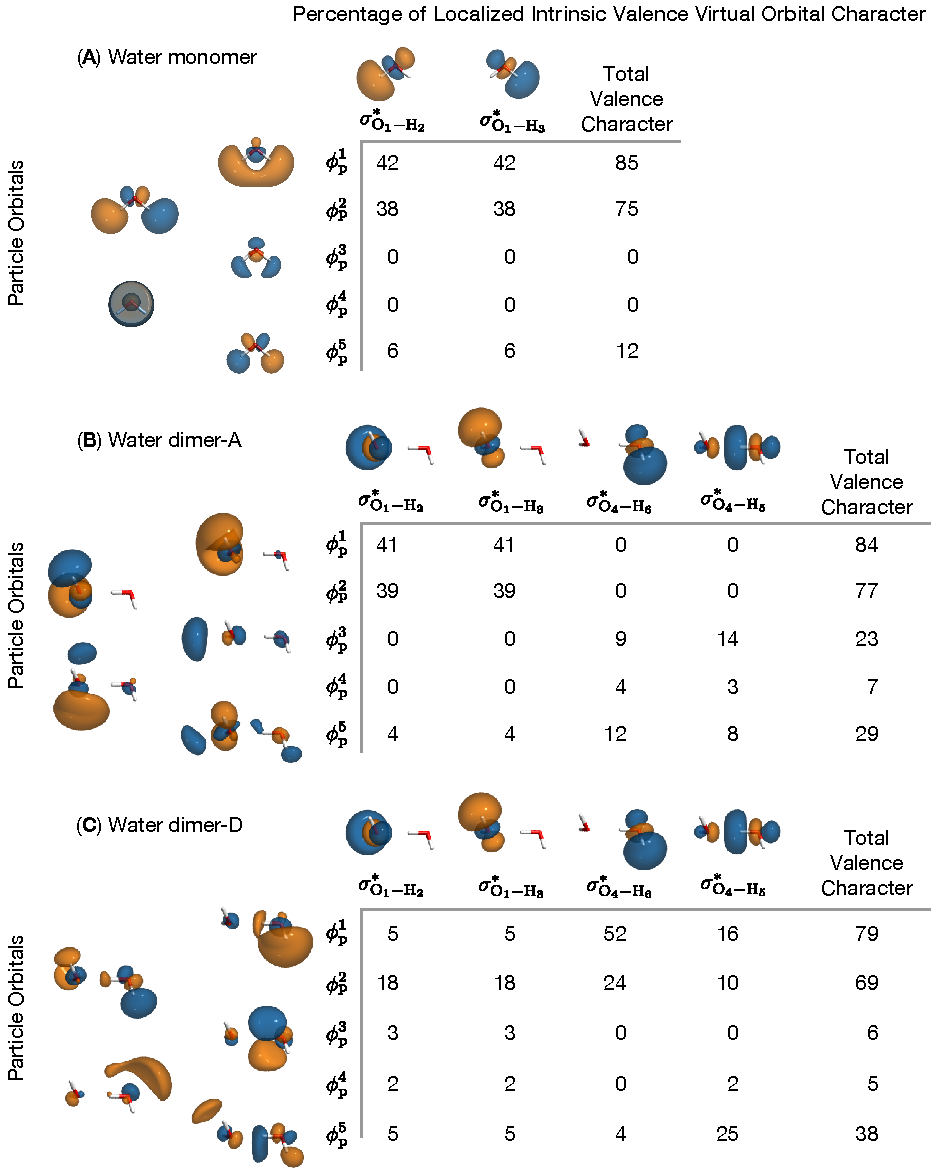
\includegraphics[width=5.75in]{figure_5_livvo_analysis_water.pdf}
\caption{Particle orbitals, valence virtual orbitals, and total valence character for each of the five core transitions in the NEXAFS spectrum of (A) water monomer, (B) the water dimer at the oxygen accepting the hydrogen bond, and (C) the water dimer at the oxygen donating the hydrogen bond.
Particle orbitals are numbered according to the calculated transitions reported in Table \ref{tab:water_spec} while atom numberings correspond to those shown in Figure~\ref{fig:water_spec}.}
\label{fig:water_all_livvo}
\end{figure*}

\textit{Water dimer, hydrogen bond donor}.
In contrast to dimer-A, the spectrum for dimer-D bears little resemblance to the monomer spectrum.
Although there are still three distinct peak features, the oscillator strength of all transitions drop significantly. We also observe a redshift of all three peaks, the first peak exhibits a mild shift of 0.2 eV while the higher energy peaks show more dramatic shifts of 0.7 and 1.0 eV respectively. The stark differences in the dimer-D spectrum, can be rationalized using our particle orbital/LIVVO analysis. The particle orbitals for each state shown in Figure~\ref{fig:water_all_livvo}C clearly show significant differences from the monomer spectrum for the dimer-D. The particle orbital for the first state in the dimer-D spectrum has similar orbital character to the first state in the monomer spectrum. However, $\phi_{\rm p}^1$ for dimer-D is clearly perturbed by the formation of the hydrogen bond and localizes along the free OH bond. 
This phenomenon has been observed in previous studies,\cite{fransson_requirements_2016,cavalleri_interpretation_2002} but the degree of localization has not been rigorously quantified. 

The LIVVO overlaps reported in Figure~\ref{fig:water_all_livvo}C for $\phi_{\rm p}^1$ shows that 52\% of the orbital character lies along the $\sigma^*_{\rm O_4-H_6}$ orbital with only 16\% localized along the hydrogen bond and 10\% of the orbital character coming from LIVVOs localized on the accepting water molecule. For $\phi_{\rm p}^2$, a similar localization is observed, however, a significantly higher percentage (36\%) of orbital character is accounted for by LIVVOs on the accepting water. This sharing of electron density with the accepting water molecule is indicative of the effect of hydrogen bonding on the dimer spectrum and has a direct correlation to the changes in intensity that we see in the simulated NEXAFS spectrum. Table \ref{tab:water_spec} shows a drop in $f_\mathrm{osc}$ when comparing the monomer to dimer-D, with a modest decrease for state 1 (0.00811 $\rightarrow$ 0.00605) and a far more drastic decrease for state 2 (0.01839 $\rightarrow$ 0.00878). This intensity drop can be attributed to delocalization of the particle orbital and correlates well with the population of LIVVOs on the accepting water molecule (10\% and 36\%, respectively).

In conclusion, LIVVOs help to address the origin behind the stark differences in the dimer-A and dimer-D spectra.
Perhaps the most revealing signature of hydrogen bonding in the water dimer is the decrease in intensity of the lowest two peaks in the dimer-D contribution.
Past studies have reasoned that the differences in these two spectra arise from the polarization of the orbitals in water.\cite{fransson_requirements_2016,cavalleri_interpretation_2002}
Due to the large dipole moment the virtual orbital are expected to be polarized toward the two hydrogen atoms and the NEXAFS spectrum will show more pronounced changes for the water molecule donating a hydrogen bond than for the one accepting it.
Our LIVVO analysis is consistent with this physical interpretation.
In addition, it quantifies the degree of delocalization of the particle orbitals in terms of localized valence orbitals.

\subsection{Basis Set Dependence of LIVVO Analysis}
An important aspect to address concerning this method is its dependence upon the choice of basis set. To fully address this issue, there are three aspects of the method that must be tested with respect to their basis set dependence: 1) How consistent are the LIVVO assignments, i.e. is there significant fluctuation in the LIVVO/IAO overlaps (eq \ref{eq:livvo_iao_overlap})? 2) Are the LIVVOs assigned to the excited state consistent? and 3) How much fluctuation is there in the particle orbital/LIVVO overlaps (eq \ref{eq:part_livvo_overlap})? We will address these three points in this section, using the two LIVVOs used to assign the first two excited states in ethanethiol, $\sigma^*_{\rm S^3-H^9}$ and $\sigma^*_{\rm S^3-C^2}$.

First we will take a look at the assignment of the atomic character of the LIVVOs, Table \ref{tab:basis_compare} shows the overlap of each VVO with eight of the IAOs in ethanethiol. These values are extremely consistent regardless of the choice of basis set, only deviating by a maximum of 0.01.

Next we will evaluate if the LIVVO assignments of the particle orbital are consistent for different basis sets. For ethanethiol, $\phi^1_{\rm p}$ was assigned primarily to the $\sigma^*_{\rm S^3-H^9}$ LIVVO with a weaker contribution from $\sigma^*_{\rm S^3-C^2}$ while $\phi^2_{\rm p}$ received a complementary assignment. Regardless of the choice of basis set, the LIVVO classification of both excited states is consistent. In all cases, $\phi^1_{\rm p}$ has greater than 57\% overlap with the  $\sigma^*_{\rm S^3-H^9}$ LIVVO and 25\% or less overlap with the $\sigma^*_{\rm S^3-C^2}$ LIVVO. Similarly, $\phi^2_{\rm p}$ has 57\% or greater overlap with $\sigma^*_{\rm S^3-C^2}$ and 25\% or less overlap with  $\sigma^*_{\rm S^3-H^9}$. The characterization of the orbital character of excited states is by far the most important feature of this technique, the consistency seen in the data across different basis sets is very encouraging. 

Lastly, we will address the consistency of the LIVVO/particle orbital overlap quantity presented in eq \ref{eq:part_livvo_overlap} with respect to choice of basis set. Table \ref{tab:basis_compare} shows that this value can potentially fluctuate $\pm$ 10\% with the choice of basis set. However, since we have shown that the formulation of the LIVVOs has a negligible dependence on the choice of basis set, we conclude that the basis set dependence seen in these values can solely be attributed to the basis set dependence of the particle orbitals.
Although these values can change fairly significantly, it is encouraging that they do not effect the overall interpretation of the excited state.

\begin{table*}[!t]
\centering
\footnotesize
\caption{Basis set dependence of the IAO assignment of LIVVOs and overlap [$\Omega_{\mathrm{p}l}^{(n)}$] of the $\sigma^*_{\rm S^3-H^9}$ and $\sigma^*_{\rm S^3-C^2}$ LIVVOs  with the first two particle orbitals of ethanethiol.}
\begin{tabular}{@{\extracolsep{6pt}}ccccccccccc@{}}
\toprule
LIVVO & $\psi^{\rm IAO}_{7}$(C$^2_{\rm s}$)& $\psi^{\rm IAO}_{9}$(C$^2_{\rm p}$)& $\psi^{\rm IAO}_{10}$(C$^2_{\rm p}$)& $\psi^{\rm IAO}_{13}$(S$^3_{\rm s}$) & $\psi^{\rm IAO}_{17}$(S$^3_{\rm p}$) & $\psi^{\rm IAO}_{18}$(S$^3_{\rm p}$) & $\psi^{\rm IAO}_{19}$(S$^3_{\rm p}$) &$\psi^{\rm IAO}_{25}$(H$^9_{\rm s}$) & $\Omega_{\mathrm{p}l}^{(1)}$ & $\Omega_{\mathrm{p}l}^{(2)}$ \\
\midrule
\multicolumn{11}{c}{\bf{cc-pVDZ}} \\
$\sigma^*_{\rm S^3-H^9}$ & 0.00 & 0.00 & 0.00 & 0.08 & 0.23 & 0.00 & 0.15 & 0.54 & 63.7 & 22.3 \\
$\sigma^*_{\rm S^3-C^2}$ & 0.09 & 0.33 & 0.09 & 0.07 & 0.00 & 0.32 & 0.09 & 0.00 & 22.6 & 67.1\\
\multicolumn{11}{c}{\bf{cc-pVTZ}} \\
$\sigma^*_{\rm S^3-H^9}$ & 0.00 & 0.00 & 0.00 & 0.08 & 0.22 & 0.00 & 0.15 & 0.54 & 59.3 & 23.9 \\
$\sigma^*_{\rm S^3-C^2}$ & 0.09 & 0.33 & 0.08 & 0.07 & 0.00 & 0.32 & 0.09 & 0.00 & 24.6 & 61.5\\
\multicolumn{11}{c}{\bf{cc-pVQZ}} \\
$\sigma^*_{\rm S^3-H^9} $& 0.00 & 0.00 & 0.00 & 0.08 & 0.22 & 0.00 & 0.15 & 0.54 & 57.8 &  22.8\\
$\sigma^*_{\rm S^3-C^2} $& 0.09 & 0.33 & 0.08 & 0.07 & 0.00 & 0.32 & 0.09 & 0.00 & 24.3 & 59.2\\
\multicolumn{11}{c}{\bf{aug-cc-pVDZ}} \\
$\sigma^*_{\rm S^3-H^9} $& 0.00 & 0.00 & 0.00 & 0.08 & 0.22 & 0.00 & 0.16 & 0.54 & 60.8 &  11.1\\
$\sigma^*_{\rm S^3-C^2} $& 0.09 & 0.33 & 0.08 & 0.07 & 0.00 & 0.32 & 0.09 & 0.00 & 15.3 & 63.1\\
\multicolumn{11}{c}{\bf{aug-cc-pVTZ}} \\
$\sigma^*_{\rm S^3-H^9} $& 0.00 & 0.00 & 0.00 & 0.08 & 0.22 & 0.00 & 0.15 & 0.54 & 57.9 &  14.7\\
$\sigma^*_{\rm S^3-C^2} $& 0.09 & 0.33 & 0.08 & 0.07 & 0.00 & 0.32 & 0.09 & 0.00 & 19.2 & 59.1\\
\multicolumn{11}{c}{\bf{aug-cc-pVQZ}} \\
$\sigma^*_{\rm S^3-H^9}$ & 0.00 & 0.00 & 0.00 & 0.07 & 0.23 & 0.00 & 0.16 & 0.54 & 56.5 & 15.7\\
$\sigma^*_{\rm S^3-C^2}$ & 0.08 & 0.33 & 0.09 & 0.07 & 0.00 & 0.32 & 0.09 & 0.00 & 20.4 & 57.3\\
\bottomrule
 \end{tabular}
 \label{tab:basis_compare}
 \end{table*}


\section{Conclusions}
In this work, we present an automated method for the characterization of core-valence excited states.
Our approach utilizes intrinsic atomic orbitals (IAOs) to derive a set of localized intrinsic valence virtual orbitals (LIVVOs) and assign their orbital character.
LIVVOs are in turn used to classify particle orbitals calculated using orthogonality constrained density functional theory (OCDFT).

For molecular orbitals with dominant valence character, this analysis provides keen insight into the localized $\sigma^*$  and $\pi^*$ orbitals that contribute to it.
For example, in the first two core excited states of ethanethiol, an electron is promoted to virtual orbitals that span both the S--C and S--H bonds. These contributions are difficult to discern by visual inspections of the MOs.
For the first state, our analysis shows that the particle orbital is dominated by the $\sigma^*_{\rm S^3-H^9}$ LIVVO (58\%) with a smaller contribution from the $\sigma^*_{\rm S^3-C^2}$ (22\%) LIVVO, revealing that this transition involves primarily the thiol bond.
Instead, for the second state we find that weights are reversed, with the $\sigma^*_{\rm S^3-C^2}$ LIVVO being the dominant contribution (57\%).

We have also shown how LIVVOs may be useful to quantify differences in excited states due to changes in the molecular environment.
For example, in the case of the water dimer we analyze the correlation between orbital localization due to hydrogen bonding and spectral features.
The NEXAFS spectrum of water dimer at the oxygen K-edge is known to have distinct contributions from the oxygens at water donating (dimer-D) or accepting (dimer-A) the hydrogen bond. 
Analysis of the two lowest particle orbitals for excitations on dimer-A show equal localization along intramolecular OH bonds.
However, the corresponding excitations for dimer-D are significantly different.
In the lowest energy state, 70\% of the electron is localized on the dimer-D, and this percentage decreases to 34\% in the second state.
These changes in degree of localization explain changes in intensity in the oxygen K-edge spectrum predicted by theory.

We have also considered the basis set dependence of the LIVVOs and the orbital analysis. Due to the robustness of the intrinsic atomic orbitals, the LIVVOs and our analysis of the orbital character are largely insensitive to the basis set size.

While our LIVVO analysis is applied here within the context of orthogonality constrained density functional theory, the method is general and can be used to decompose any set of virtual orbitals.
Overall, our LIVVO-based analysis of particle orbitals is a first step toward creating a general, robust, and automatic method to assign the character of excited states.

\newpage

\section*{Acknowledgments}
This work was supported by start-up funds provided by Emory University.
We would like to thank  Dr. Robert M. Parrish for kindly providing us with the implementation of intrinsic atomic orbitals in Psi4.
W.D.D. is supported by the National Science Foundation Graduate Research Fellowship under Grant No. 0000048655. Any opinion, findings, and conclusions or recommendations expressed in this material are those of the authors and do not necessarily reflect the views of the National Science Foundation.


{\footnotesize
\bibliography{refs}
\bibliographystyle{achemso}
}
\end{document}
